%\documentclass[10pt]{beamer}
\documentclass[hyperref={pdfpagemode=FullScreen},aspectratio=169,10pt]{beamer}
\usetheme[subsectionpage=progressbar]{metropolis}
\setbeamertemplate{section in toc}[sections numbered]
\setbeamertemplate{subsection in toc}[subsections numbered]
\metroset{progressbar=frametitle}
\metroset{numbering=none}
%W\usepackage[utf8]{inputenc}
\usepackage{ragged2e}
\usepackage{caption}
\usepackage{amsmath}
\usepackage[mathrm=sym]{unicode-math}
\setmathfont{Fira Math}
\usepackage{graphicx} 
\usepackage{outlines}
\usepackage{appendixnumberbeamer}
\usepackage{booktabs}
\usepackage[font=small,labelfont=bf]{caption}
\usepackage{hyperref}
\usepackage[scale=2]{ccicons}
\usepackage{caption}
\usepackage{subcaption}
\graphicspath{{../figures/}}
\usepackage{pgfplots}
\usepgfplotslibrary{dateplot}
\setsansfont[BoldFont={Fira Sans Bold}]{Fira Sans Book}
\usepackage{xspace}
\newcommand{\themename}{\textbf{\textsc{metropolis}}\xspace}
\theoremstyle{definition}
\metroset{block=fill}

\definecolor{Purple}{HTML}{911146}
\definecolor{Orange}{HTML}{CF4A30}
\setbeamercolor{alerted text}{fg=Orange}
\setbeamercolor{frametitle}{bg=Orange}
\renewcommand<>{\alert}[1]{\begin{alertenv}\bfseries#2#1\end{alertenv}}


\title{Detecting influential beliefs in large-scale surveys}
\date{July 2021}
\author{Aleksandar Tomašević}
\institute{University of Novi Sad}
%\titlegraphic{\hfill\includegraphics[height=1.9cm]{ff.pdf}}
\hbadness=99999
\begin{document}
\begin{frame}
    \titlepage
\end{frame}


  \begin{frame}
  \tableofcontents[hideallsubsections]
  \end{frame}


\section{Research problem}

\begin{frame}{Belief systems in large-scale surveys}
\large
\begin{flushleft}
  \begin{itemize}
    \item<+-> \alert{Large-scale} surveys?
    \item<+-> \textit{ESS, GSS, ALLBUS, BSAS}
    \item<+-> \alert{Belief system} construction
    \item<+-> \alert{Influential beliefs?}
  \end{itemize}

\end{flushleft}

\end{frame}

\begin{frame}{Motivating example - ESS - Attitude towards government}
  \begin{columns}[T] % align columns
    \begin{column}{.48\textwidth}

    \begin{block}{Govermental Performance}
      Satisfaction with \alert{Economy} \\
      Satisfaction with \alert{Democracy} \\
      State of \alert{Healthcare}  \\
      State of \alert{Education}  
    \end{block}

    \vspace{0.5cm}

    \begin{block}{Political Trust}
      \alert{Parliament} \\
      \alert{Legal system} \\
      \alert{Police}  \\
      \alert{Politicians}  \\ 
      \alert{Political parties} 
    \end{block}
    
    \end{column}%
    \hfill%
    \begin{column}{.48\textwidth}
      \begin{block}{Representation \& Fairness}
        Systems allows people to have \alert{a say} \\
        Systems allows people to have \alert{influence}  \\
        Gov. decisions are \alert{transparent}   \\
        Gov. takes into account \alert{interests of all}  \\ 
        System gives a \alert{fair chance} to all
      \end{block}
    \end{column}%
    \end{columns}
\end{frame}

\begin{frame}{Analytical strategy}
  \begin{outline}
  \1 CAN - UVA - IVI
  \1 GGM with redundancy analysis (UVA)
  \1 Network tree - partition of covariance matrix of GGM
  \1 Centrality - Influence - IVI
  \1 IVI differences between groups
  \end{outline}
\end{frame}
\section{Belief networks}

{\setbeamercolor{background canvas}{bg=white} \begin{frame}
  \begin{flushleft}
  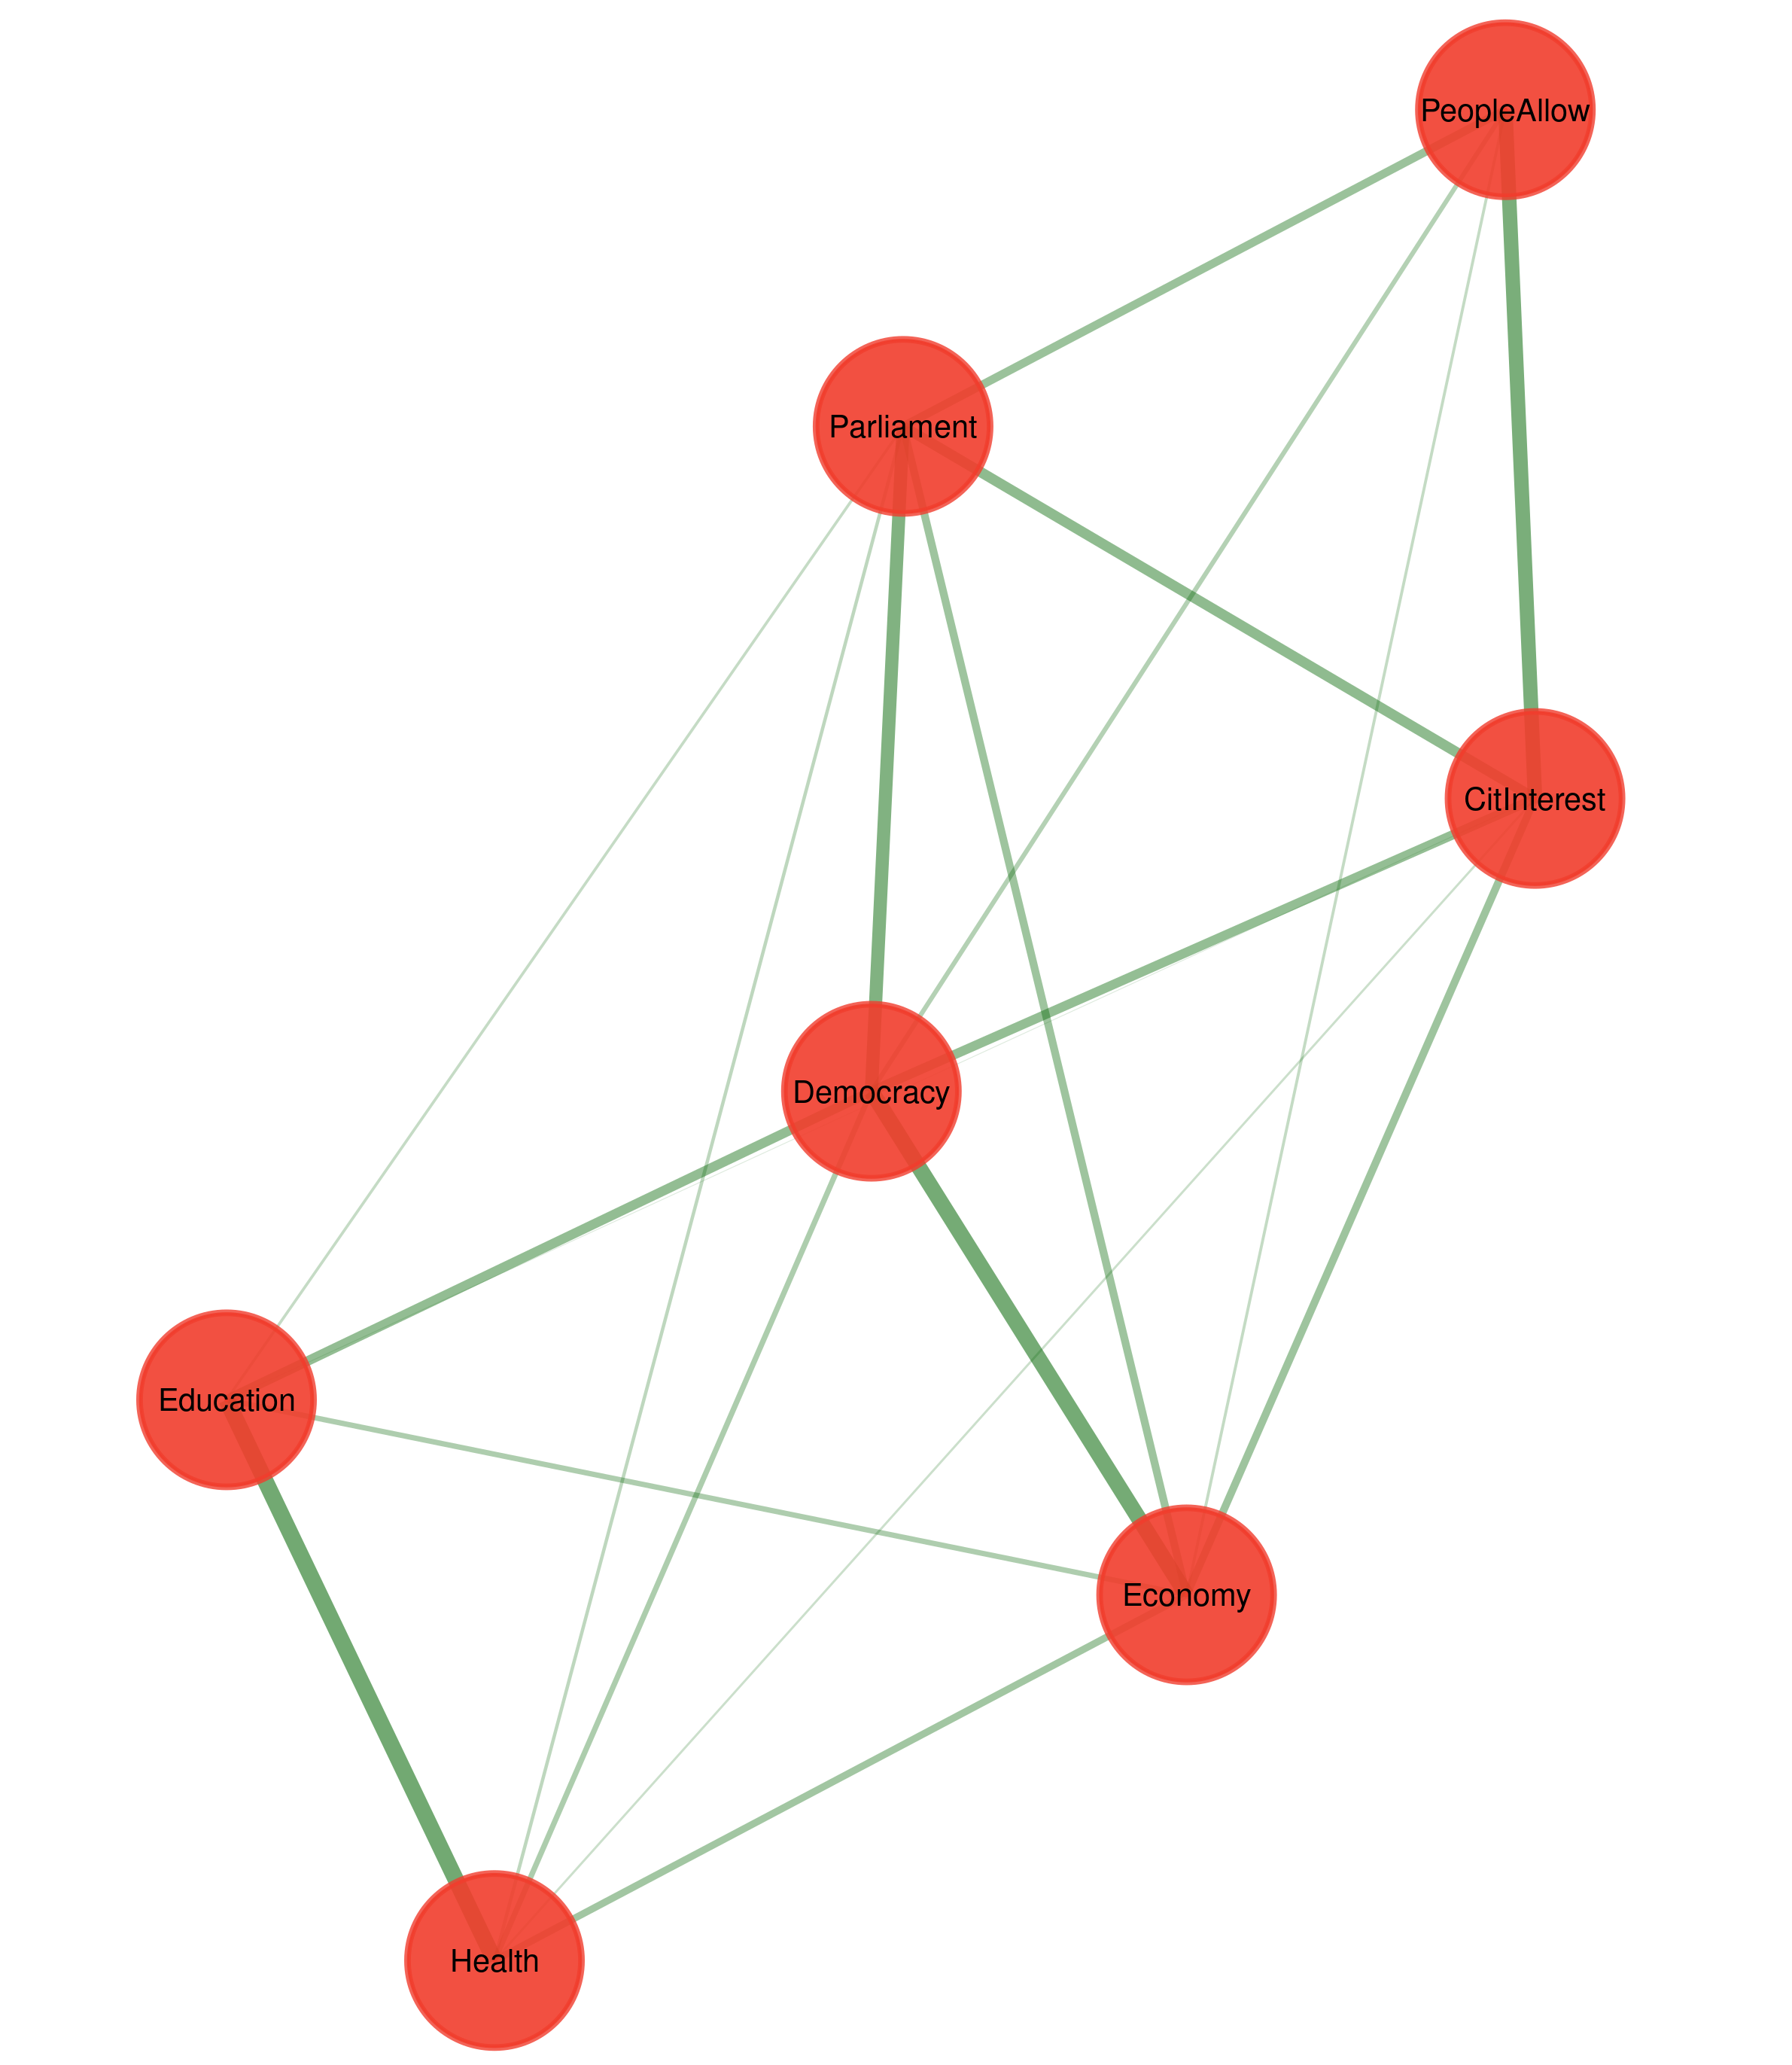
\includegraphics[width=0.5\paperwidth]{01-ega-full.png}
  \end{flushleft}
\end{frame}}

{\setbeamercolor{background canvas}{bg=white} \begin{frame}{\hspace{0.5cm}Electoral autocracies \hspace{0.5cm} VS \hspace{0.5cm} Liberal Democracies}
  \begin{figure}
  \begin{flushleft}
  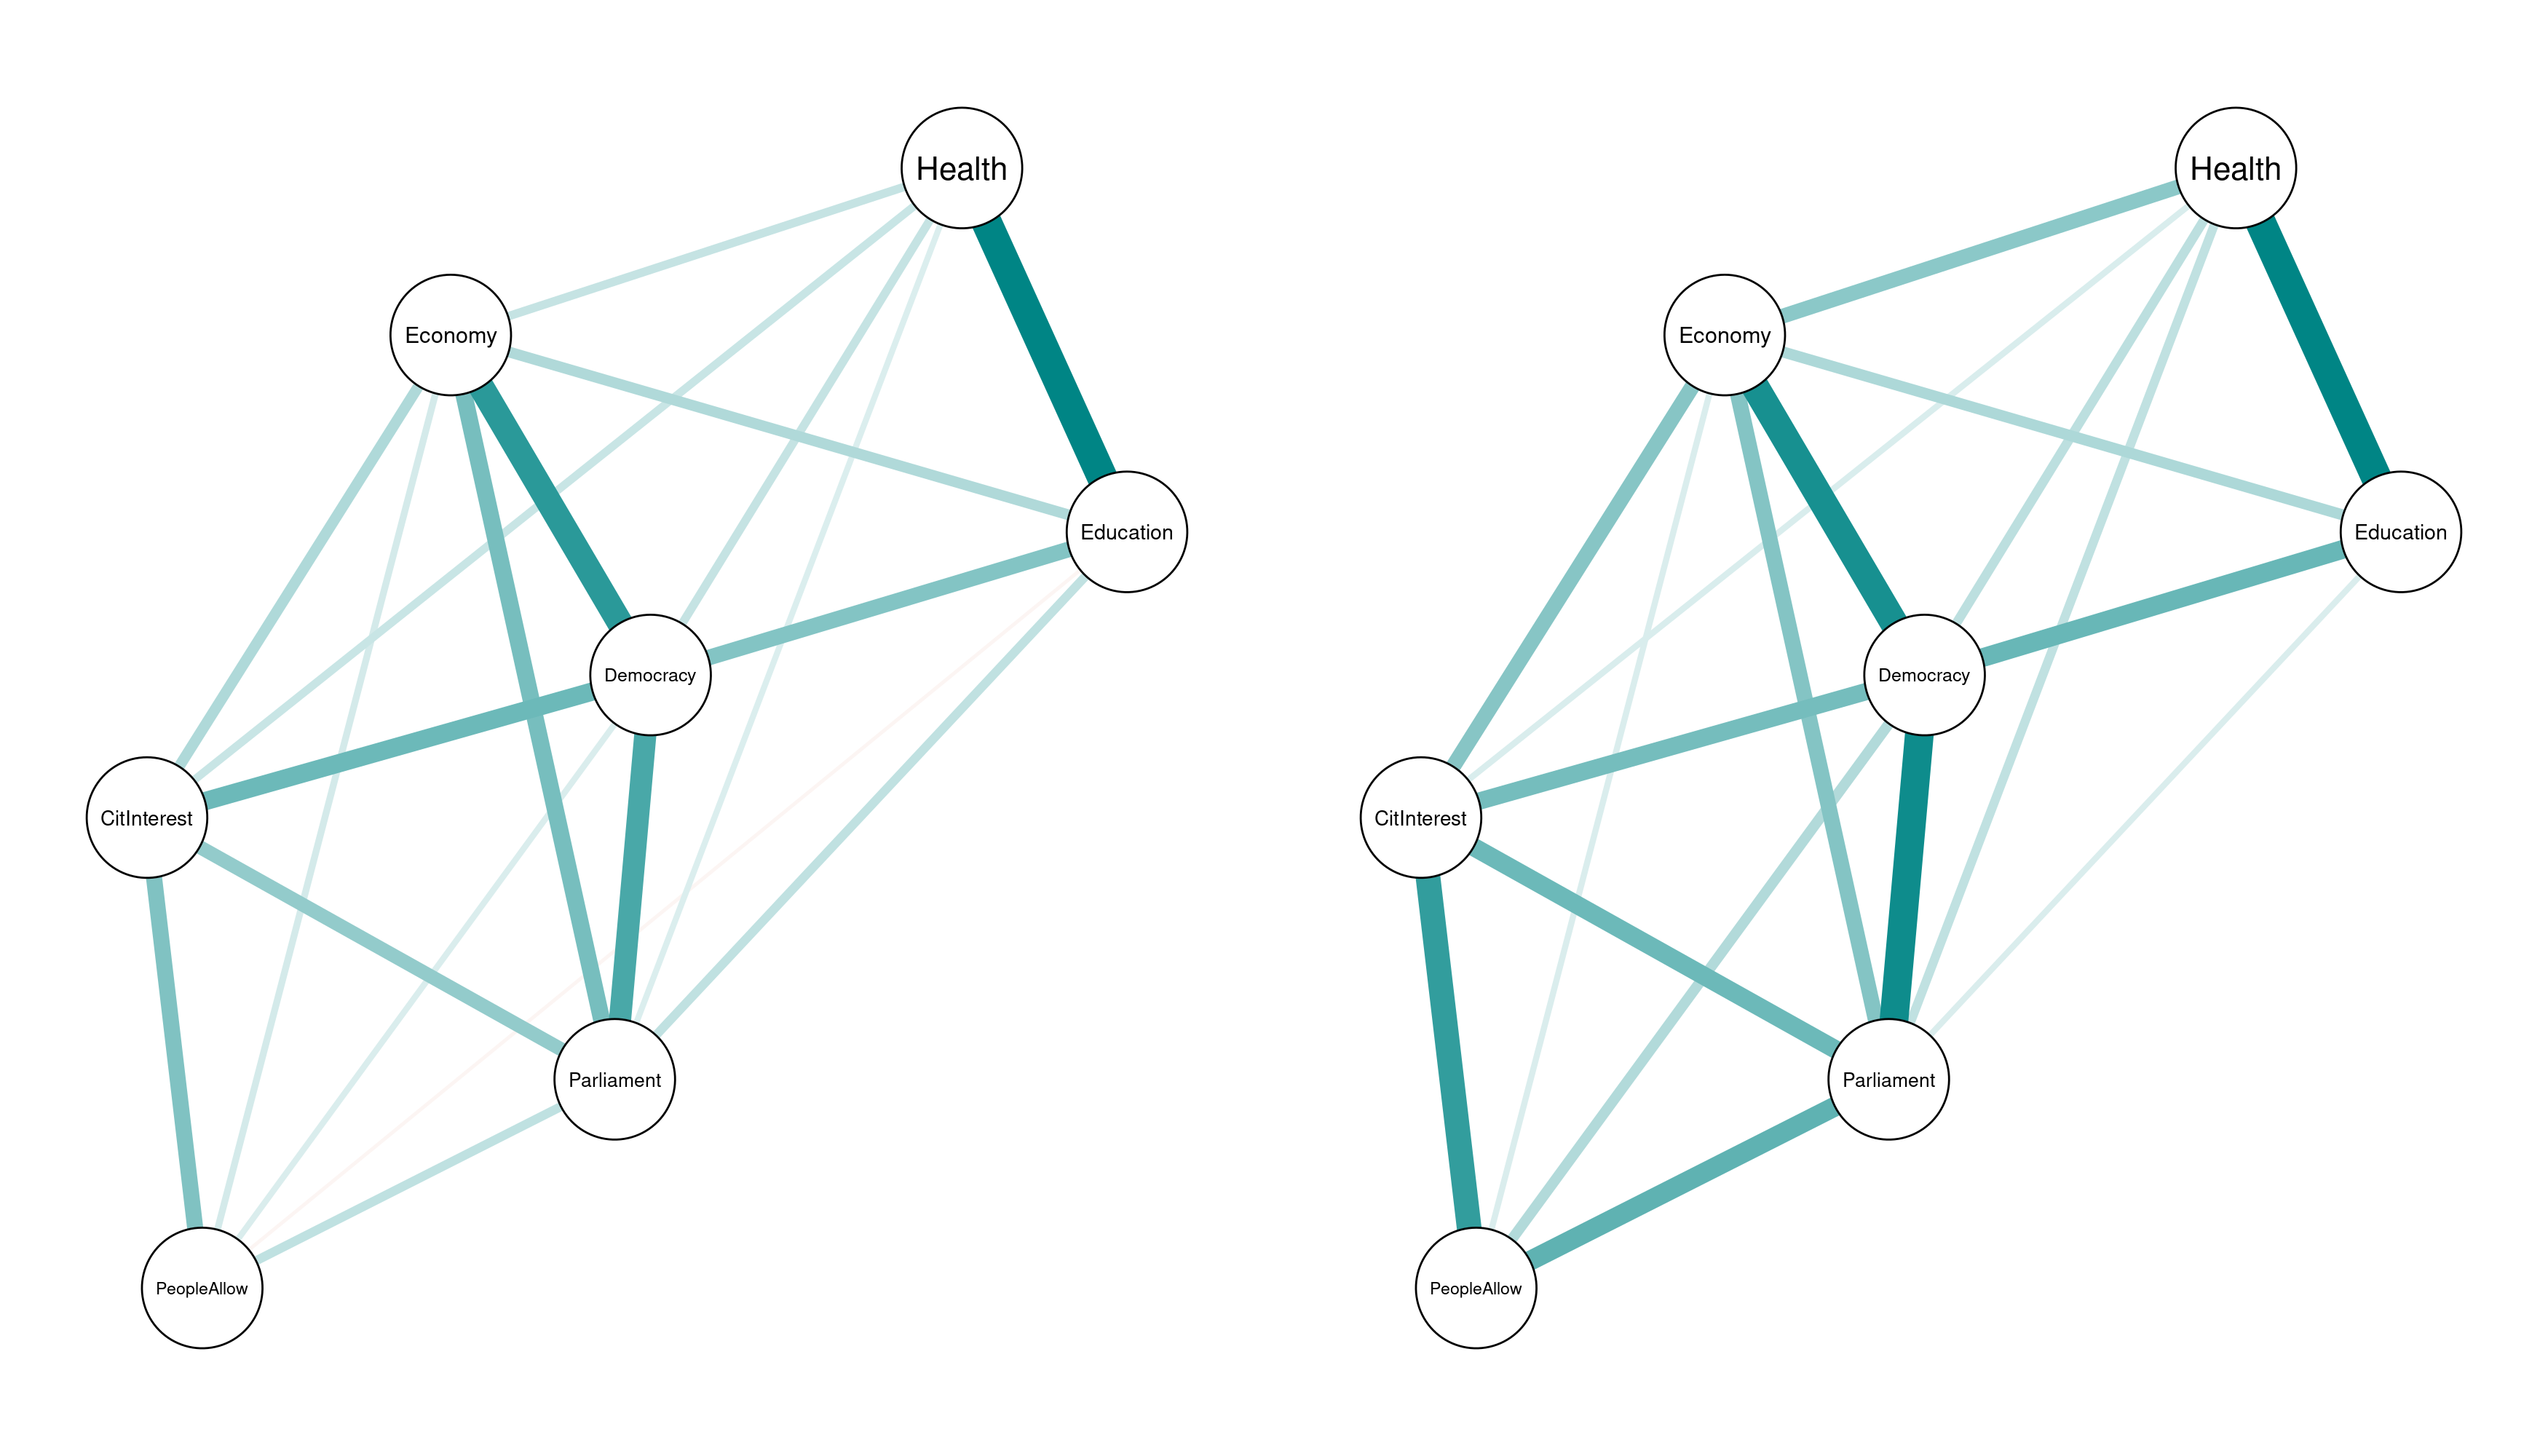
\includegraphics[width=0.75\paperwidth]{99-tree-ea-vs-ld.png}
  \end{flushleft}
  \end{figure}
\end{frame}}

\section{Integrated Value of Influence}

{\setbeamercolor{background canvas}{bg=white} \begin{frame}
  \begin{figure}
  \begin{flushleft}
  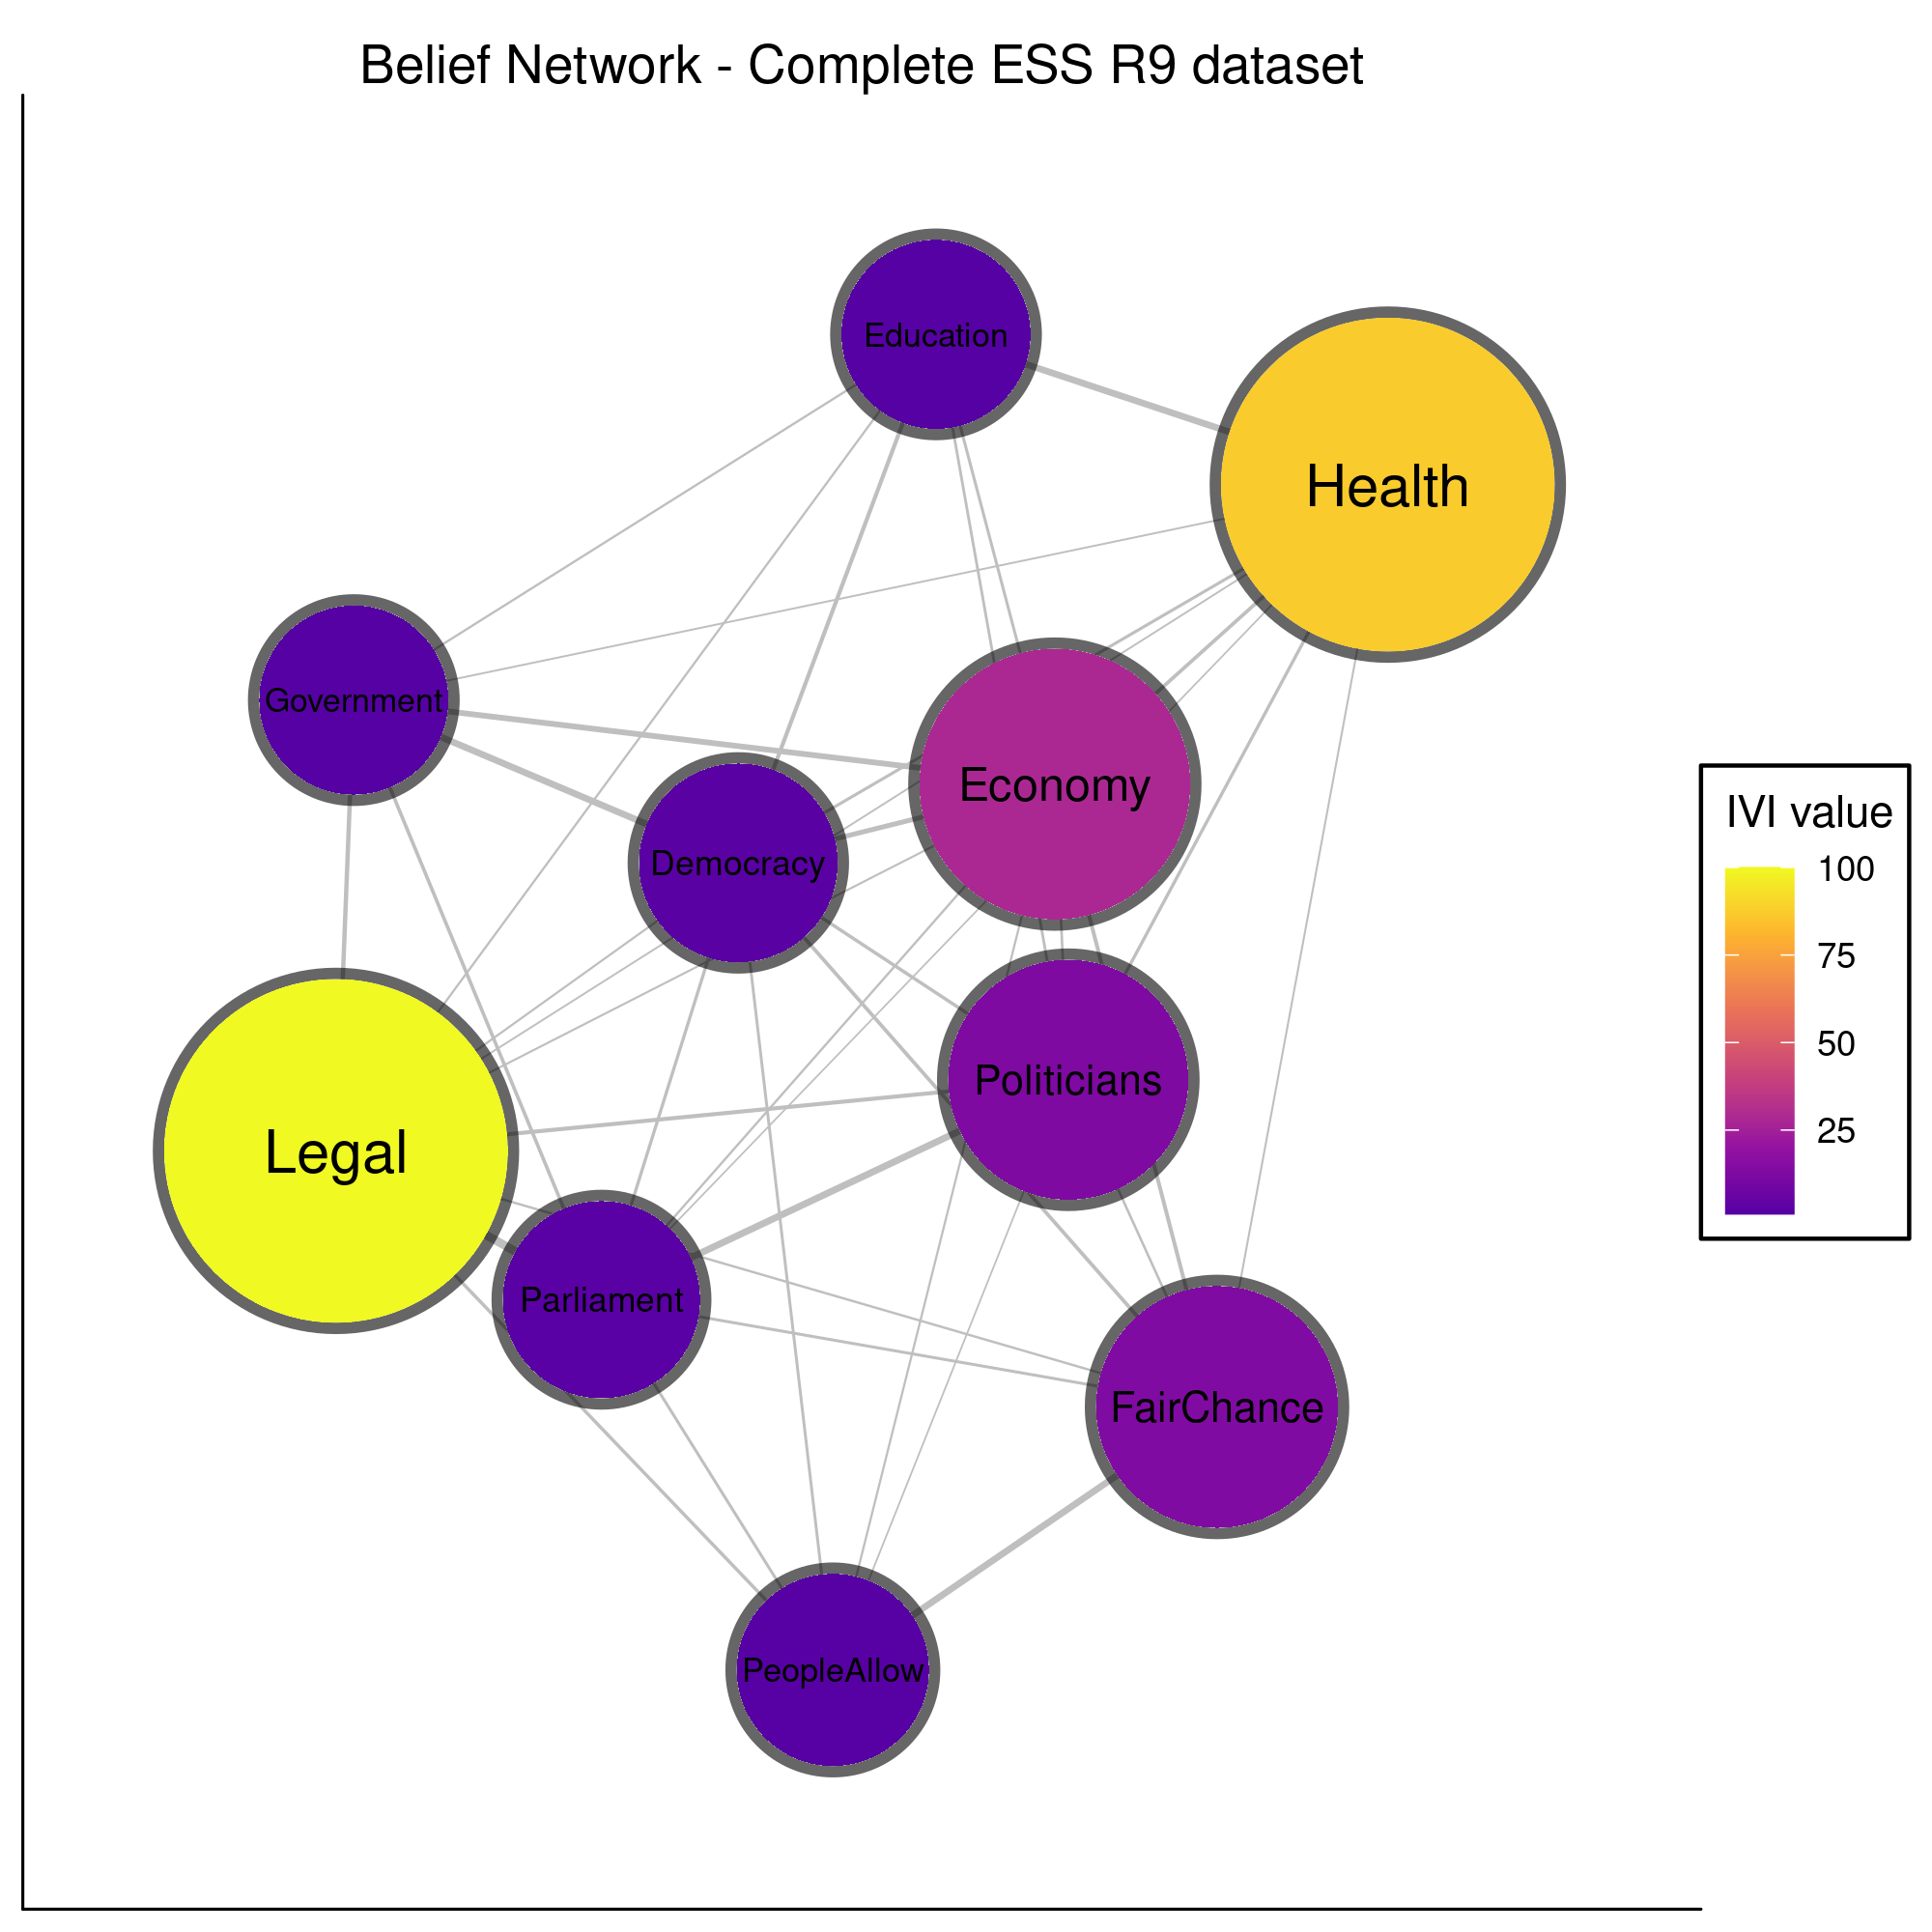
\includegraphics[width=0.6\paperwidth]{02-ivi-full.png}
  \end{flushleft}

  \end{figure}
\end{frame}}

{\setbeamercolor{background canvas}{bg=white} \begin{frame}
  \begin{figure}
  \begin{flushleft}
  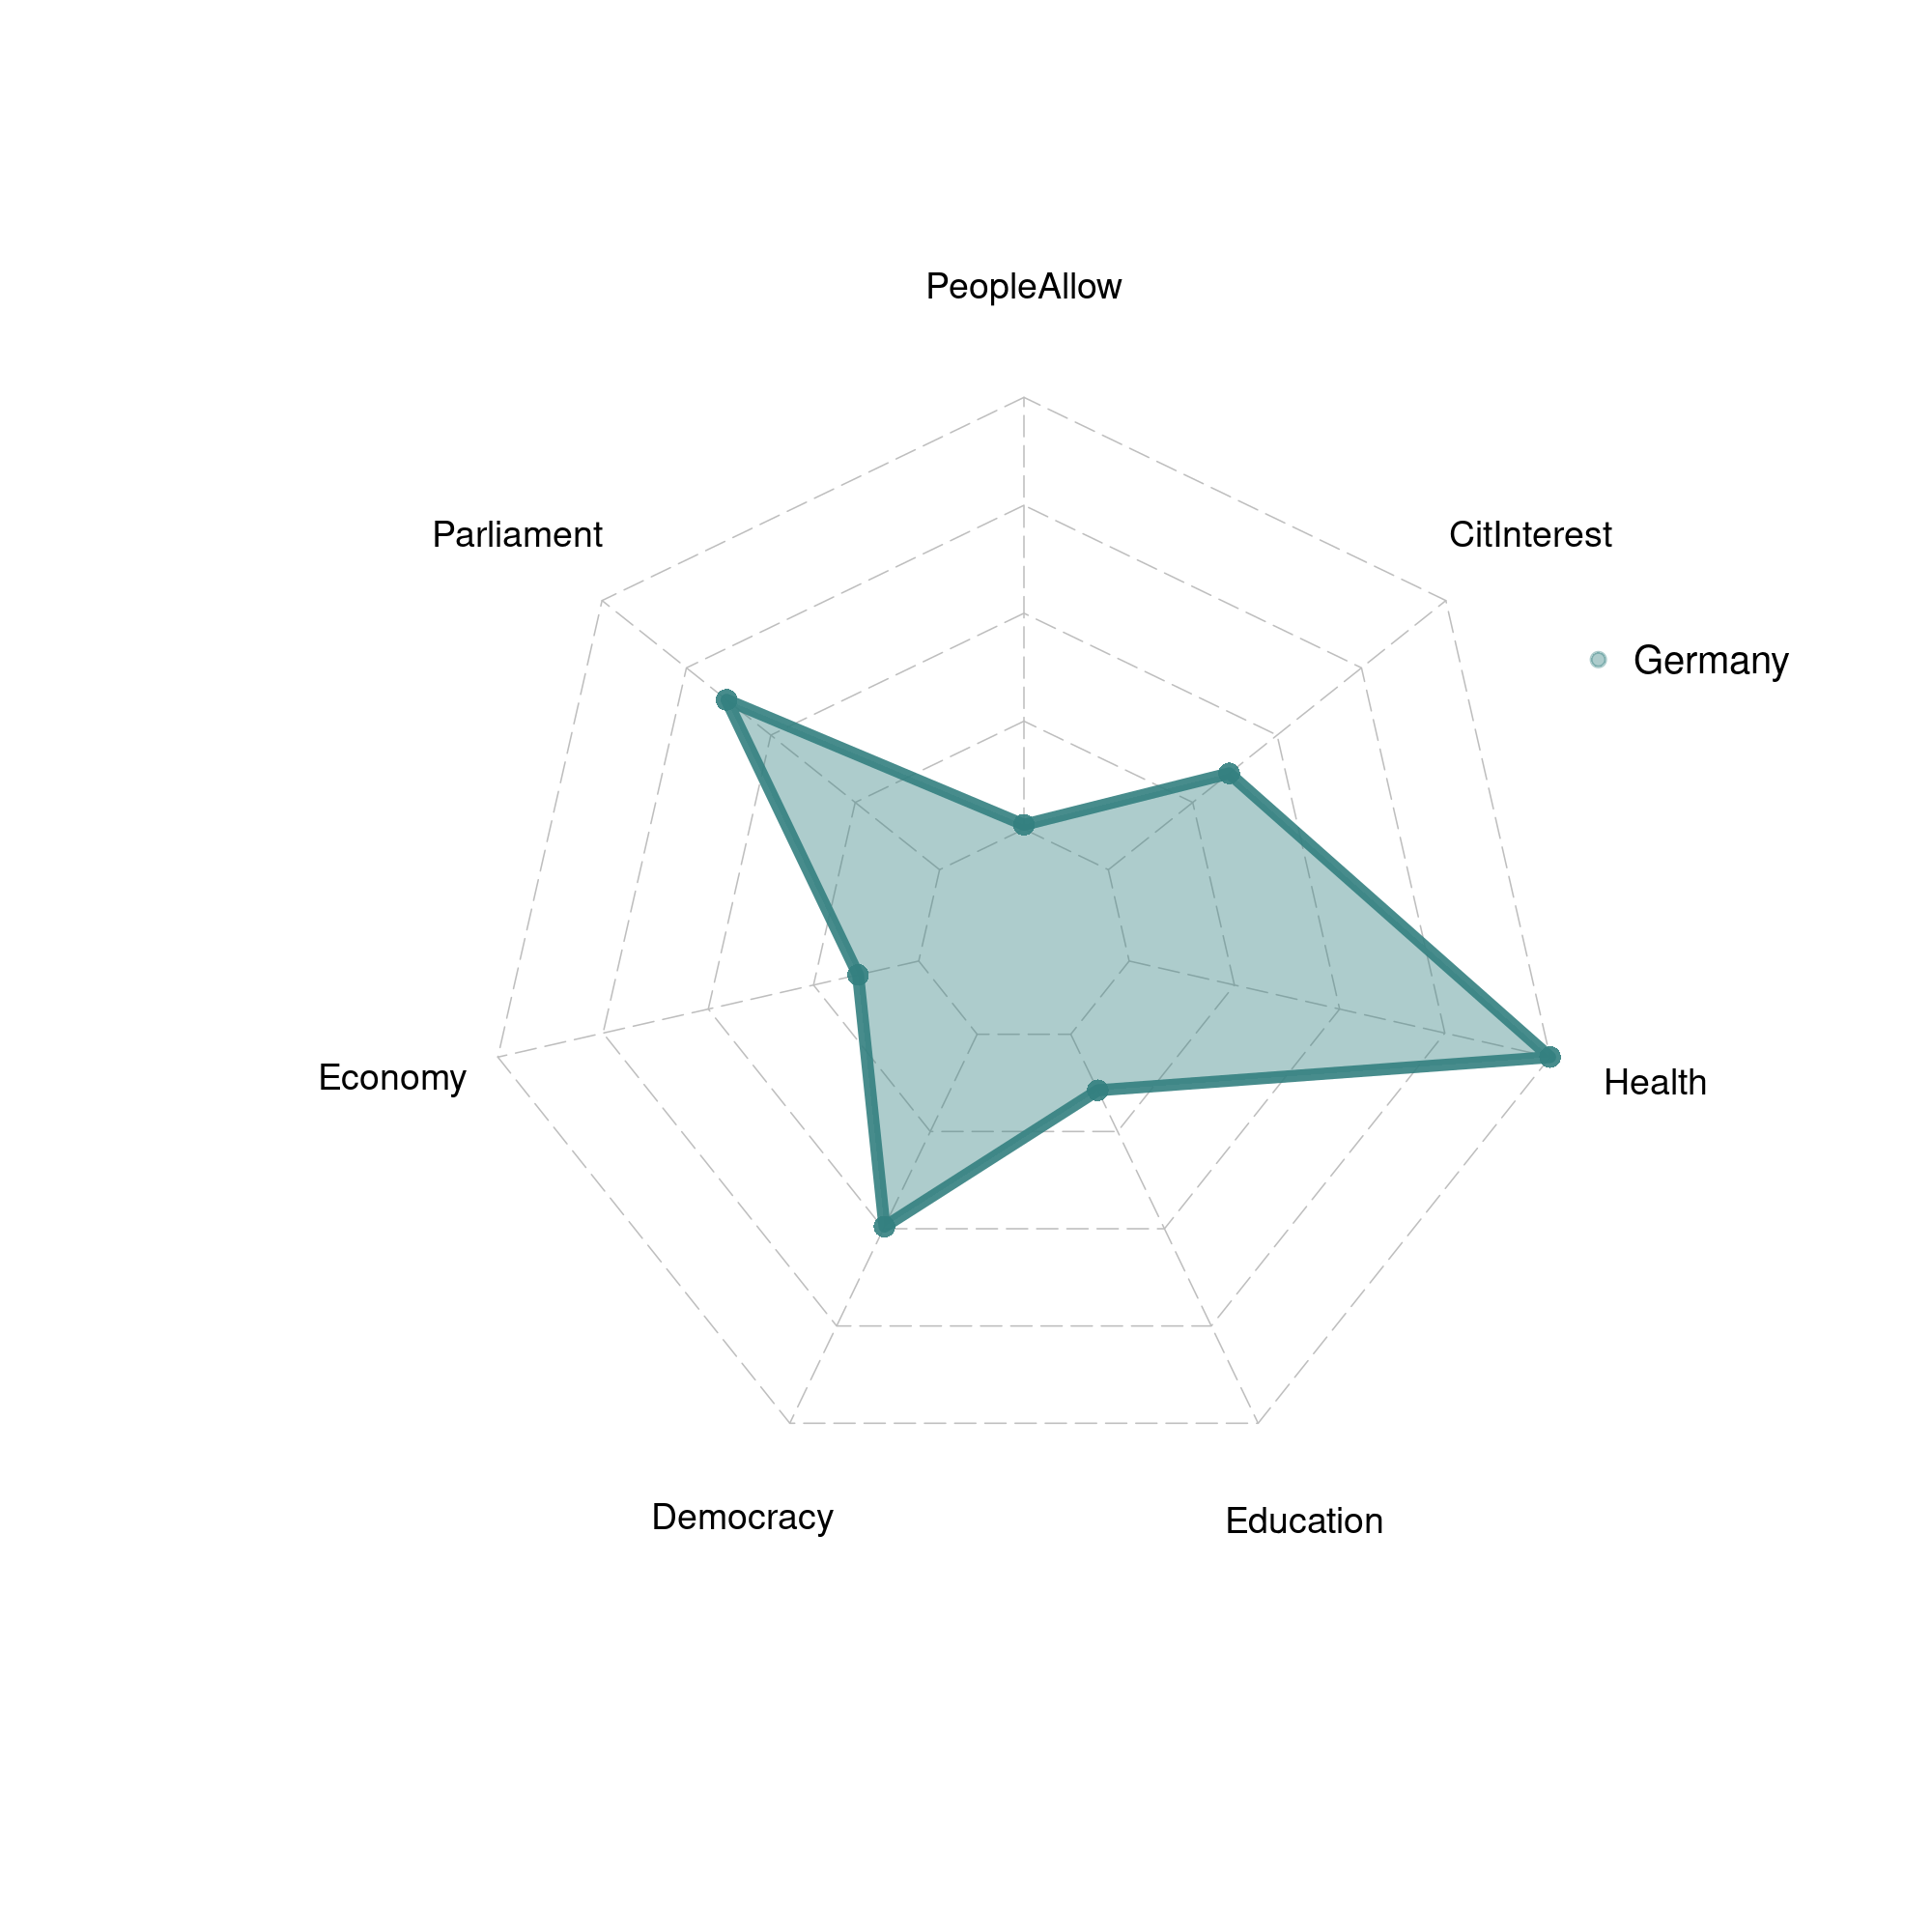
\includegraphics[width=0.65\paperwidth]{03-radar-ger.png}
  \end{flushleft}

  \end{figure}
\end{frame}}

{\setbeamercolor{background canvas}{bg=white} \begin{frame}
  \begin{figure}
    \begin{flushleft}
    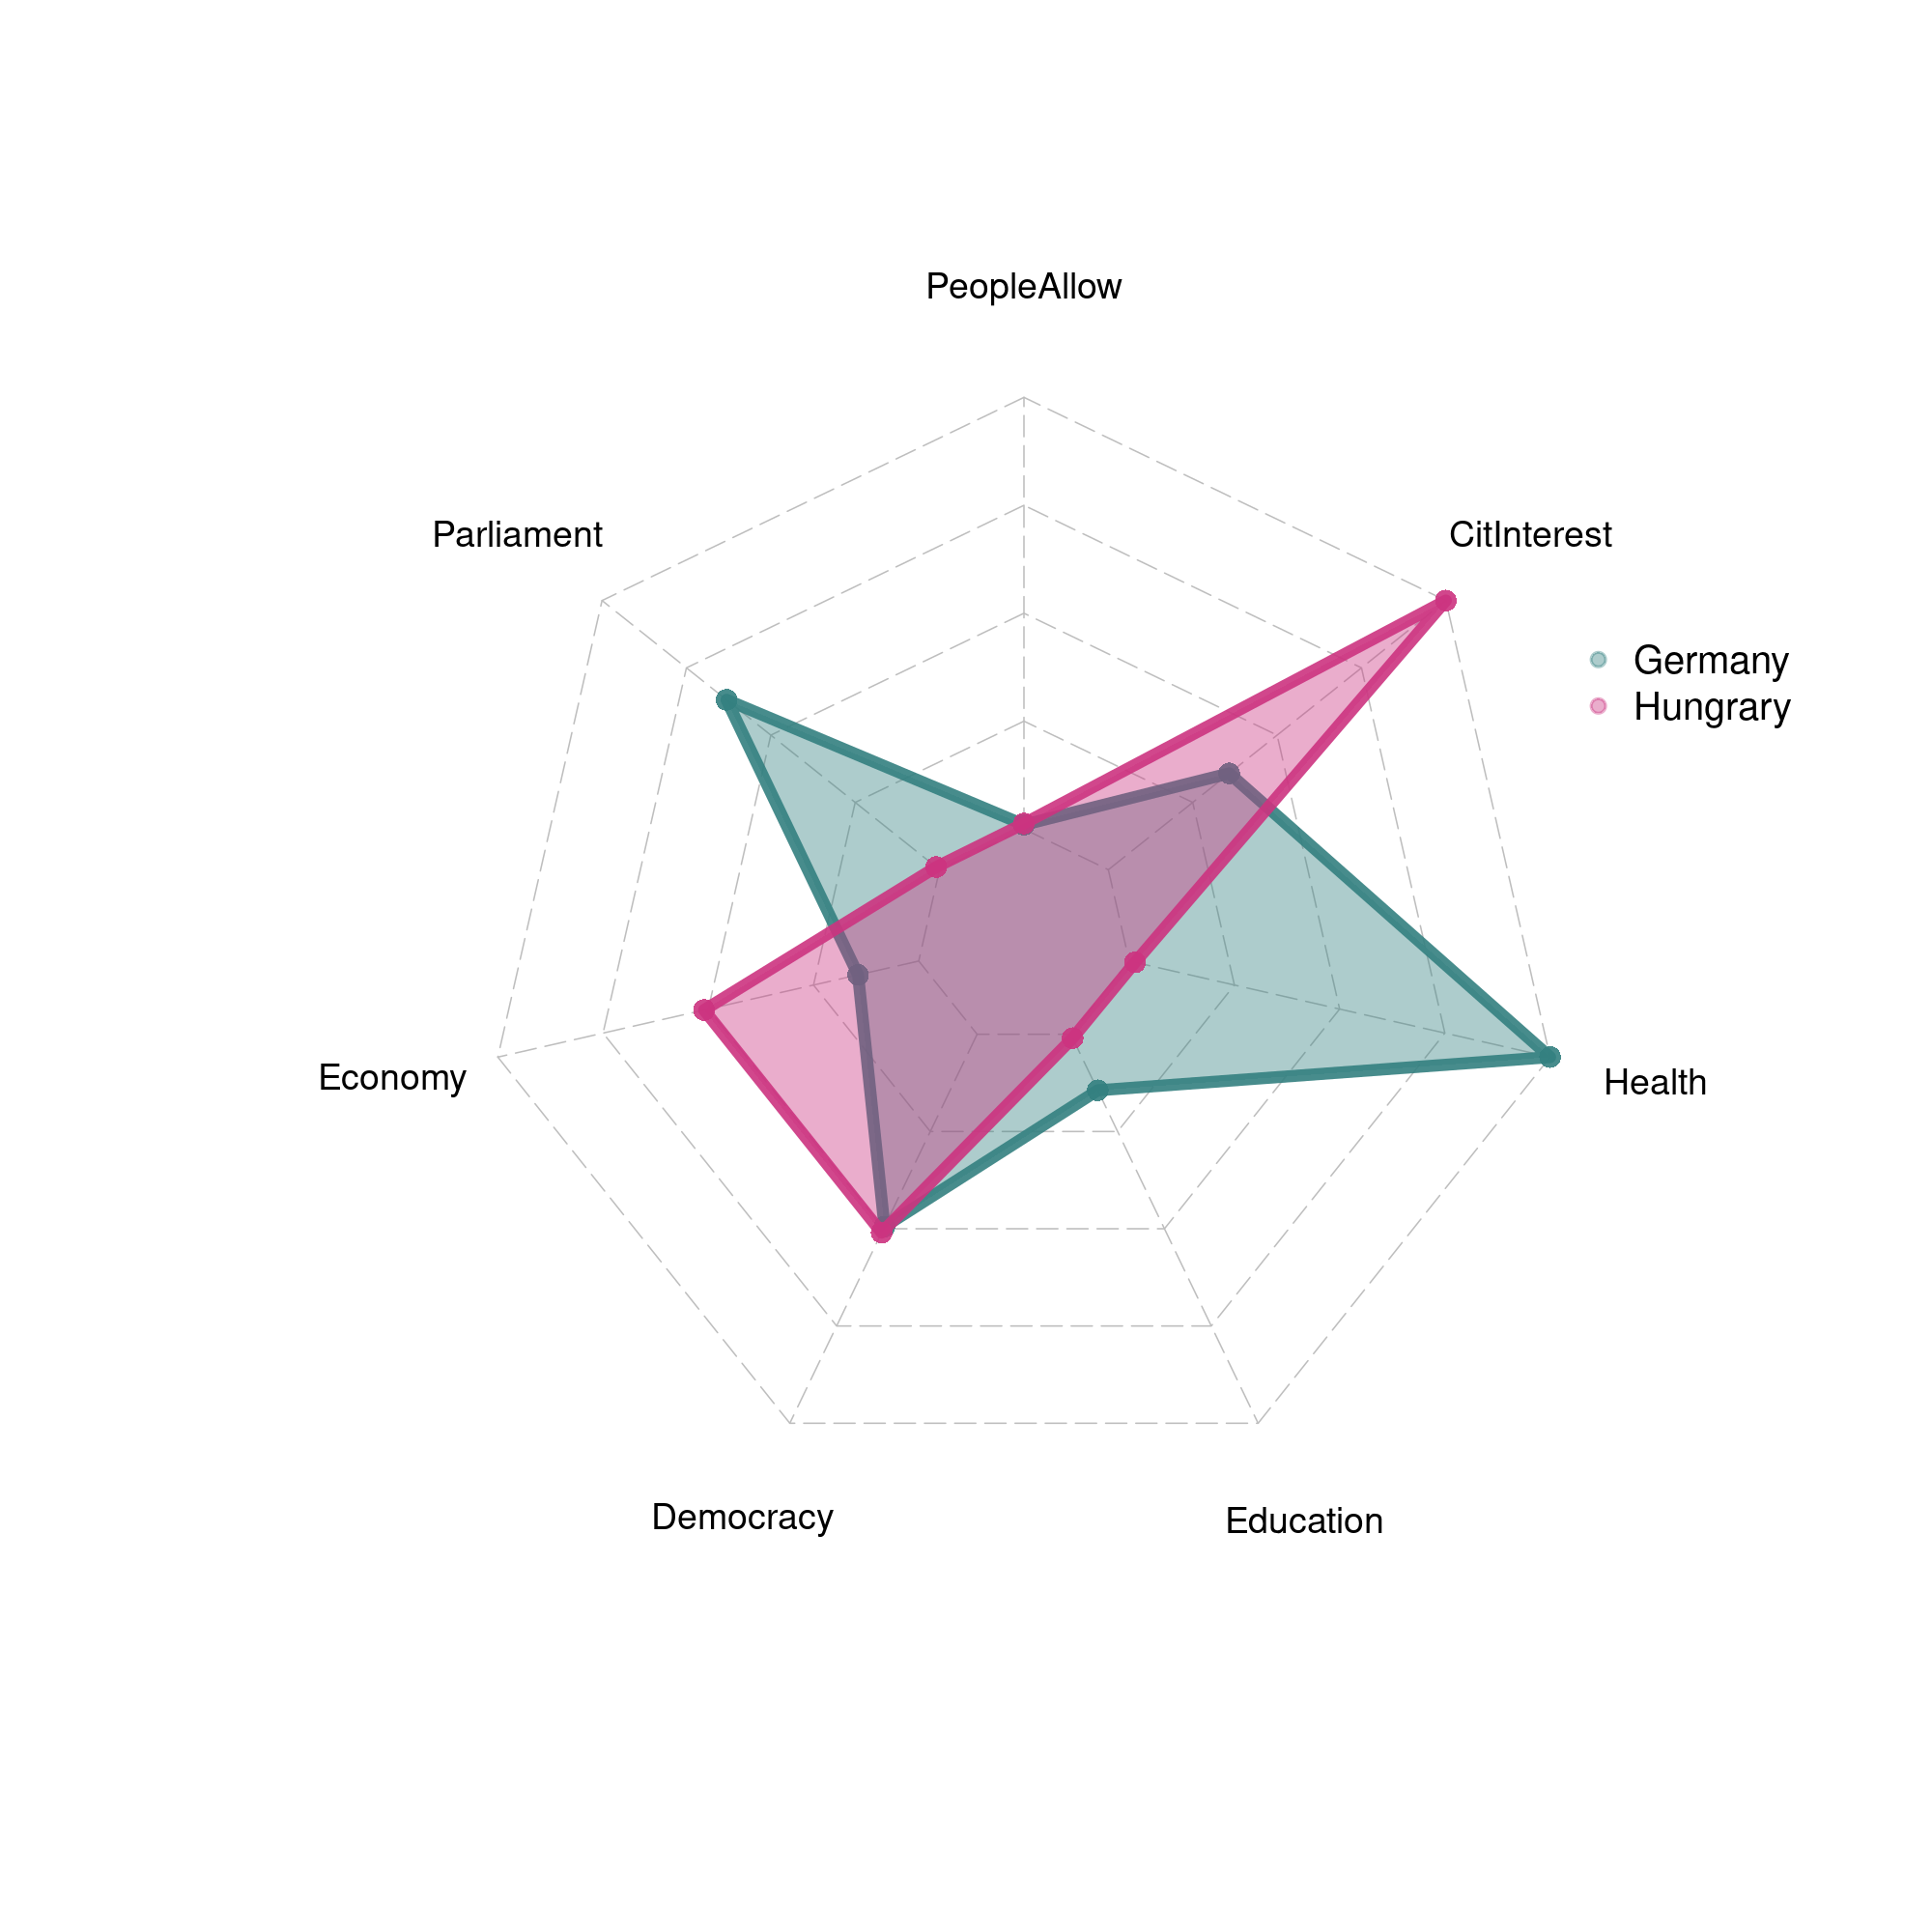
\includegraphics[width=0.65\paperwidth]{03-radar-ger-hu.png}
    \end{flushleft}
    \end{figure}
\end{frame}}

\setbeamercolor{background canvas}{bg=white}

\begin{frame}
  \begin{figure}
    \begin{flushleft}
    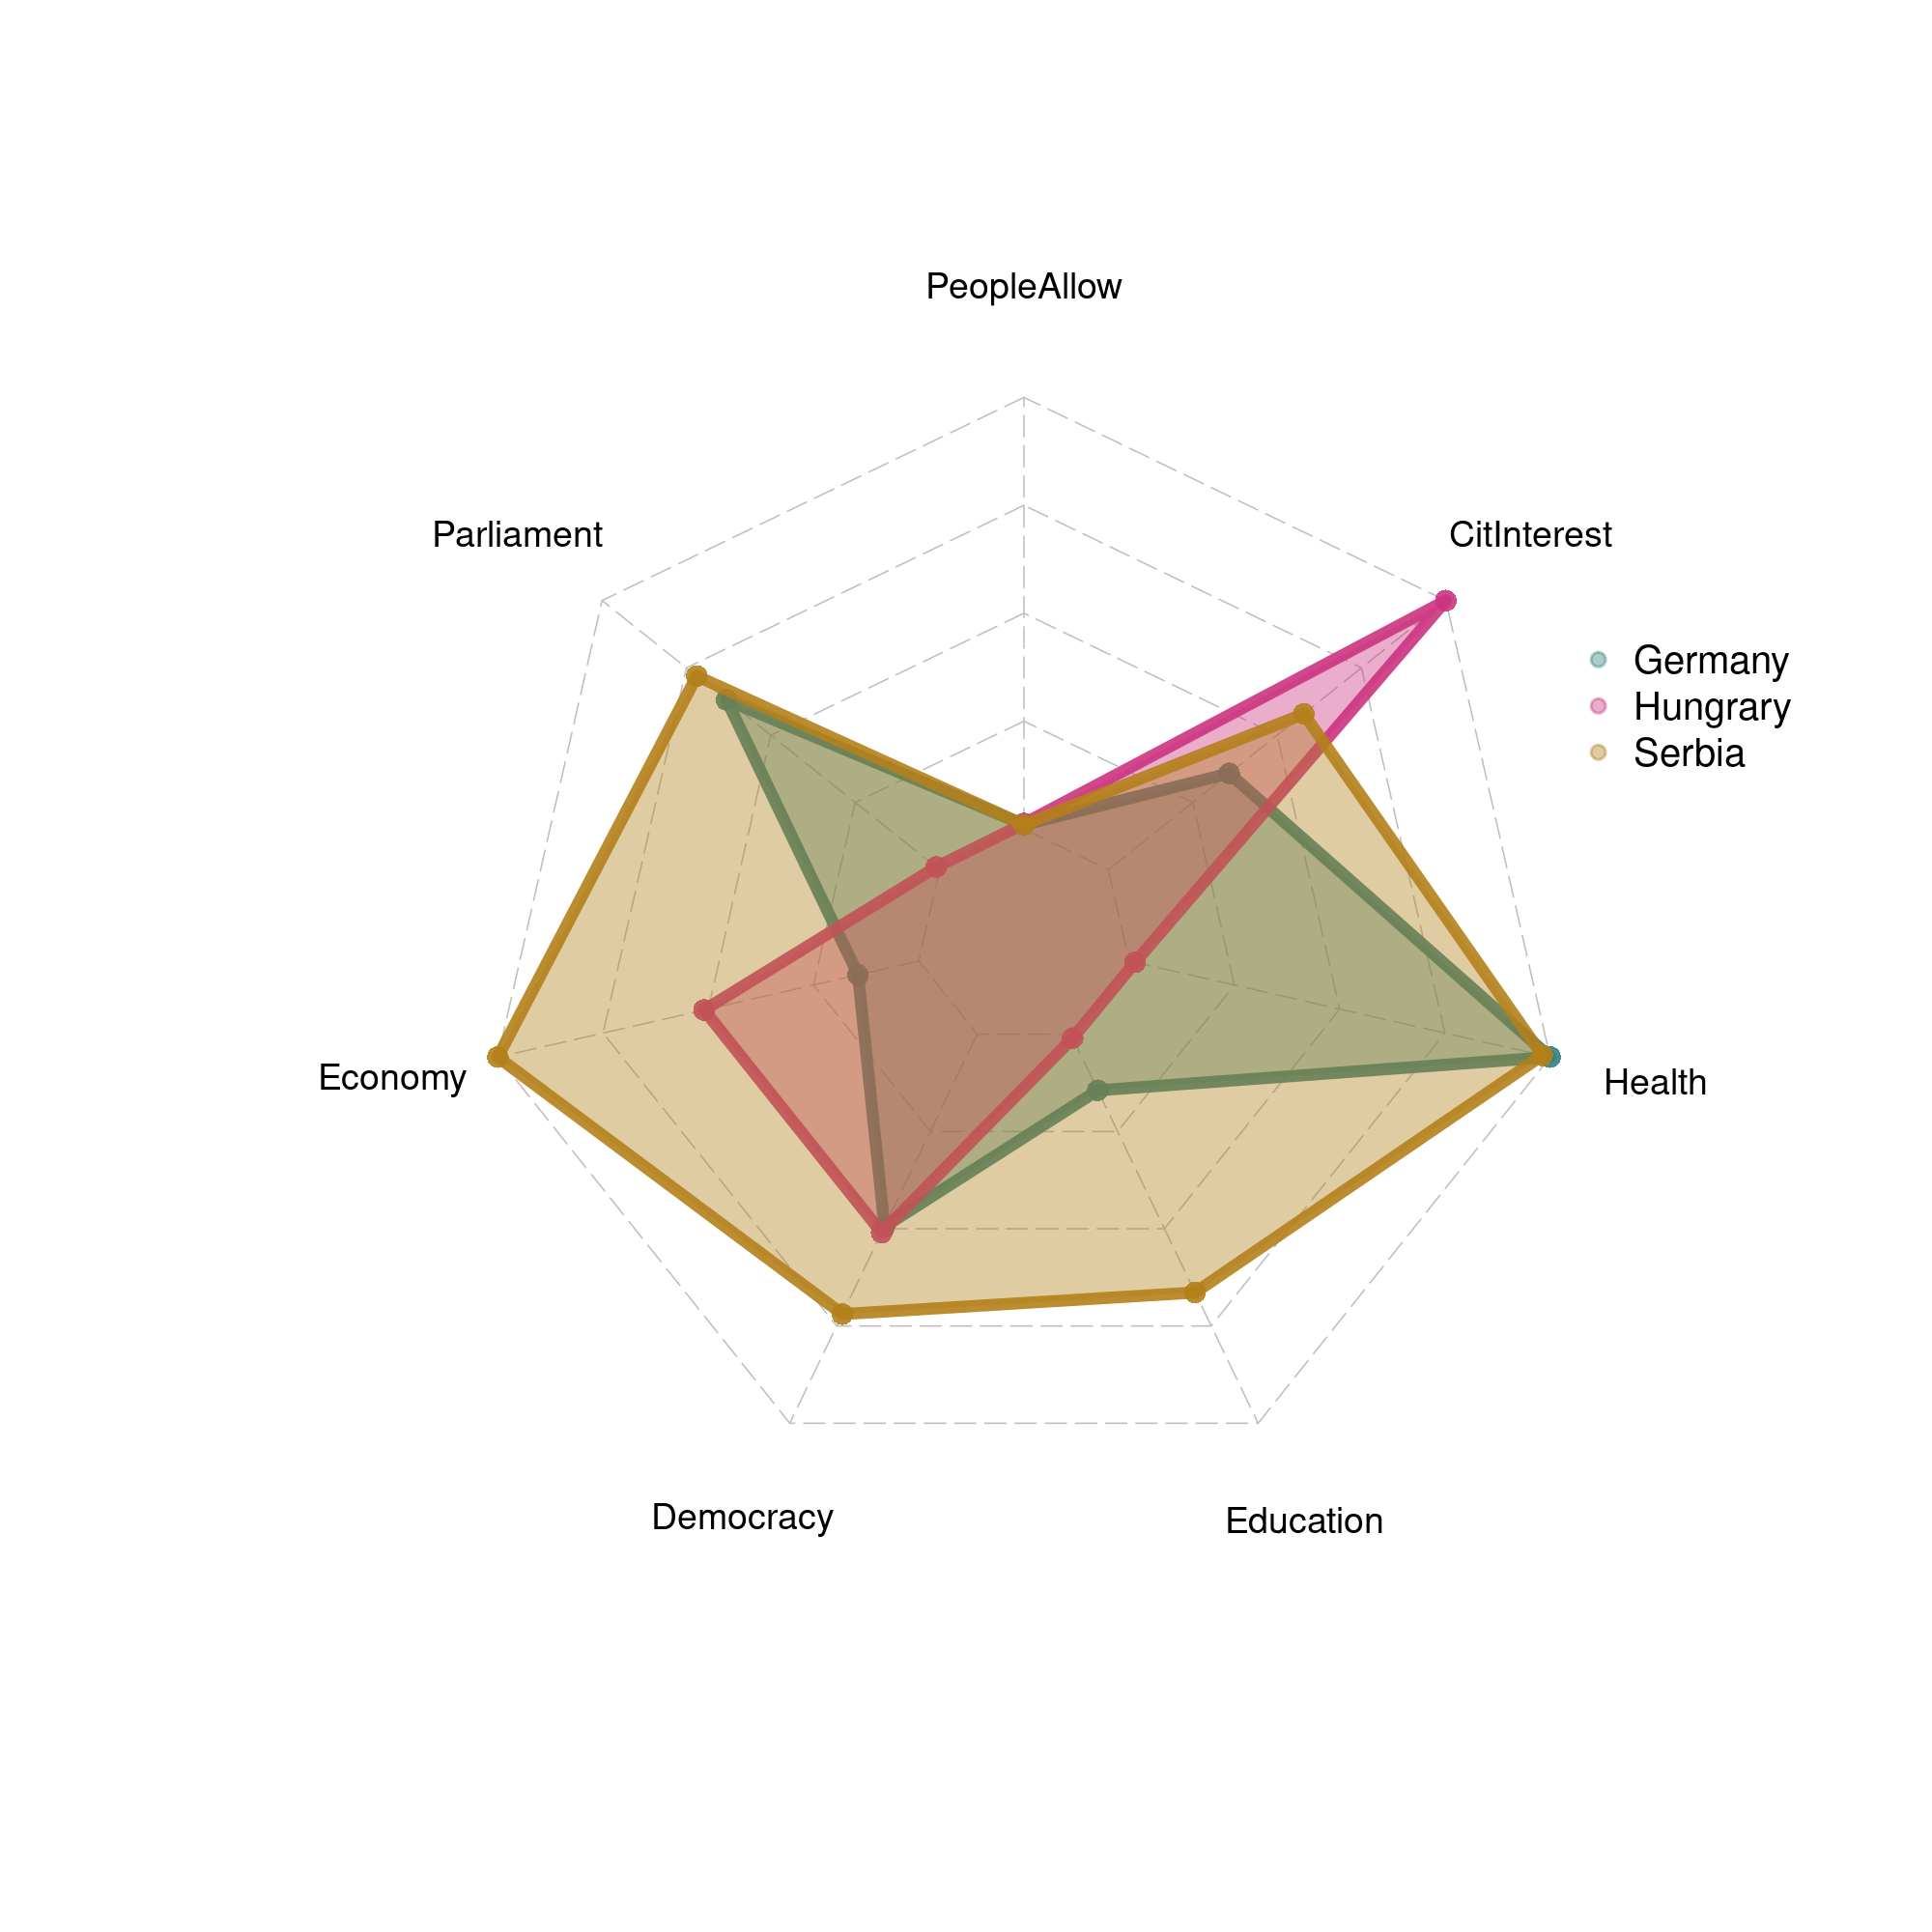
\includegraphics[width=0.65\paperwidth]{03-radar-hu-rs.png}
    \end{flushleft}
    \end{figure}
\end{frame}

\setbeamercolor{background canvas}{bg=white} 
\begin{frame}{GDP per capita vs Economy IVI}
  \begin{figure}
    \begin{flushleft}

  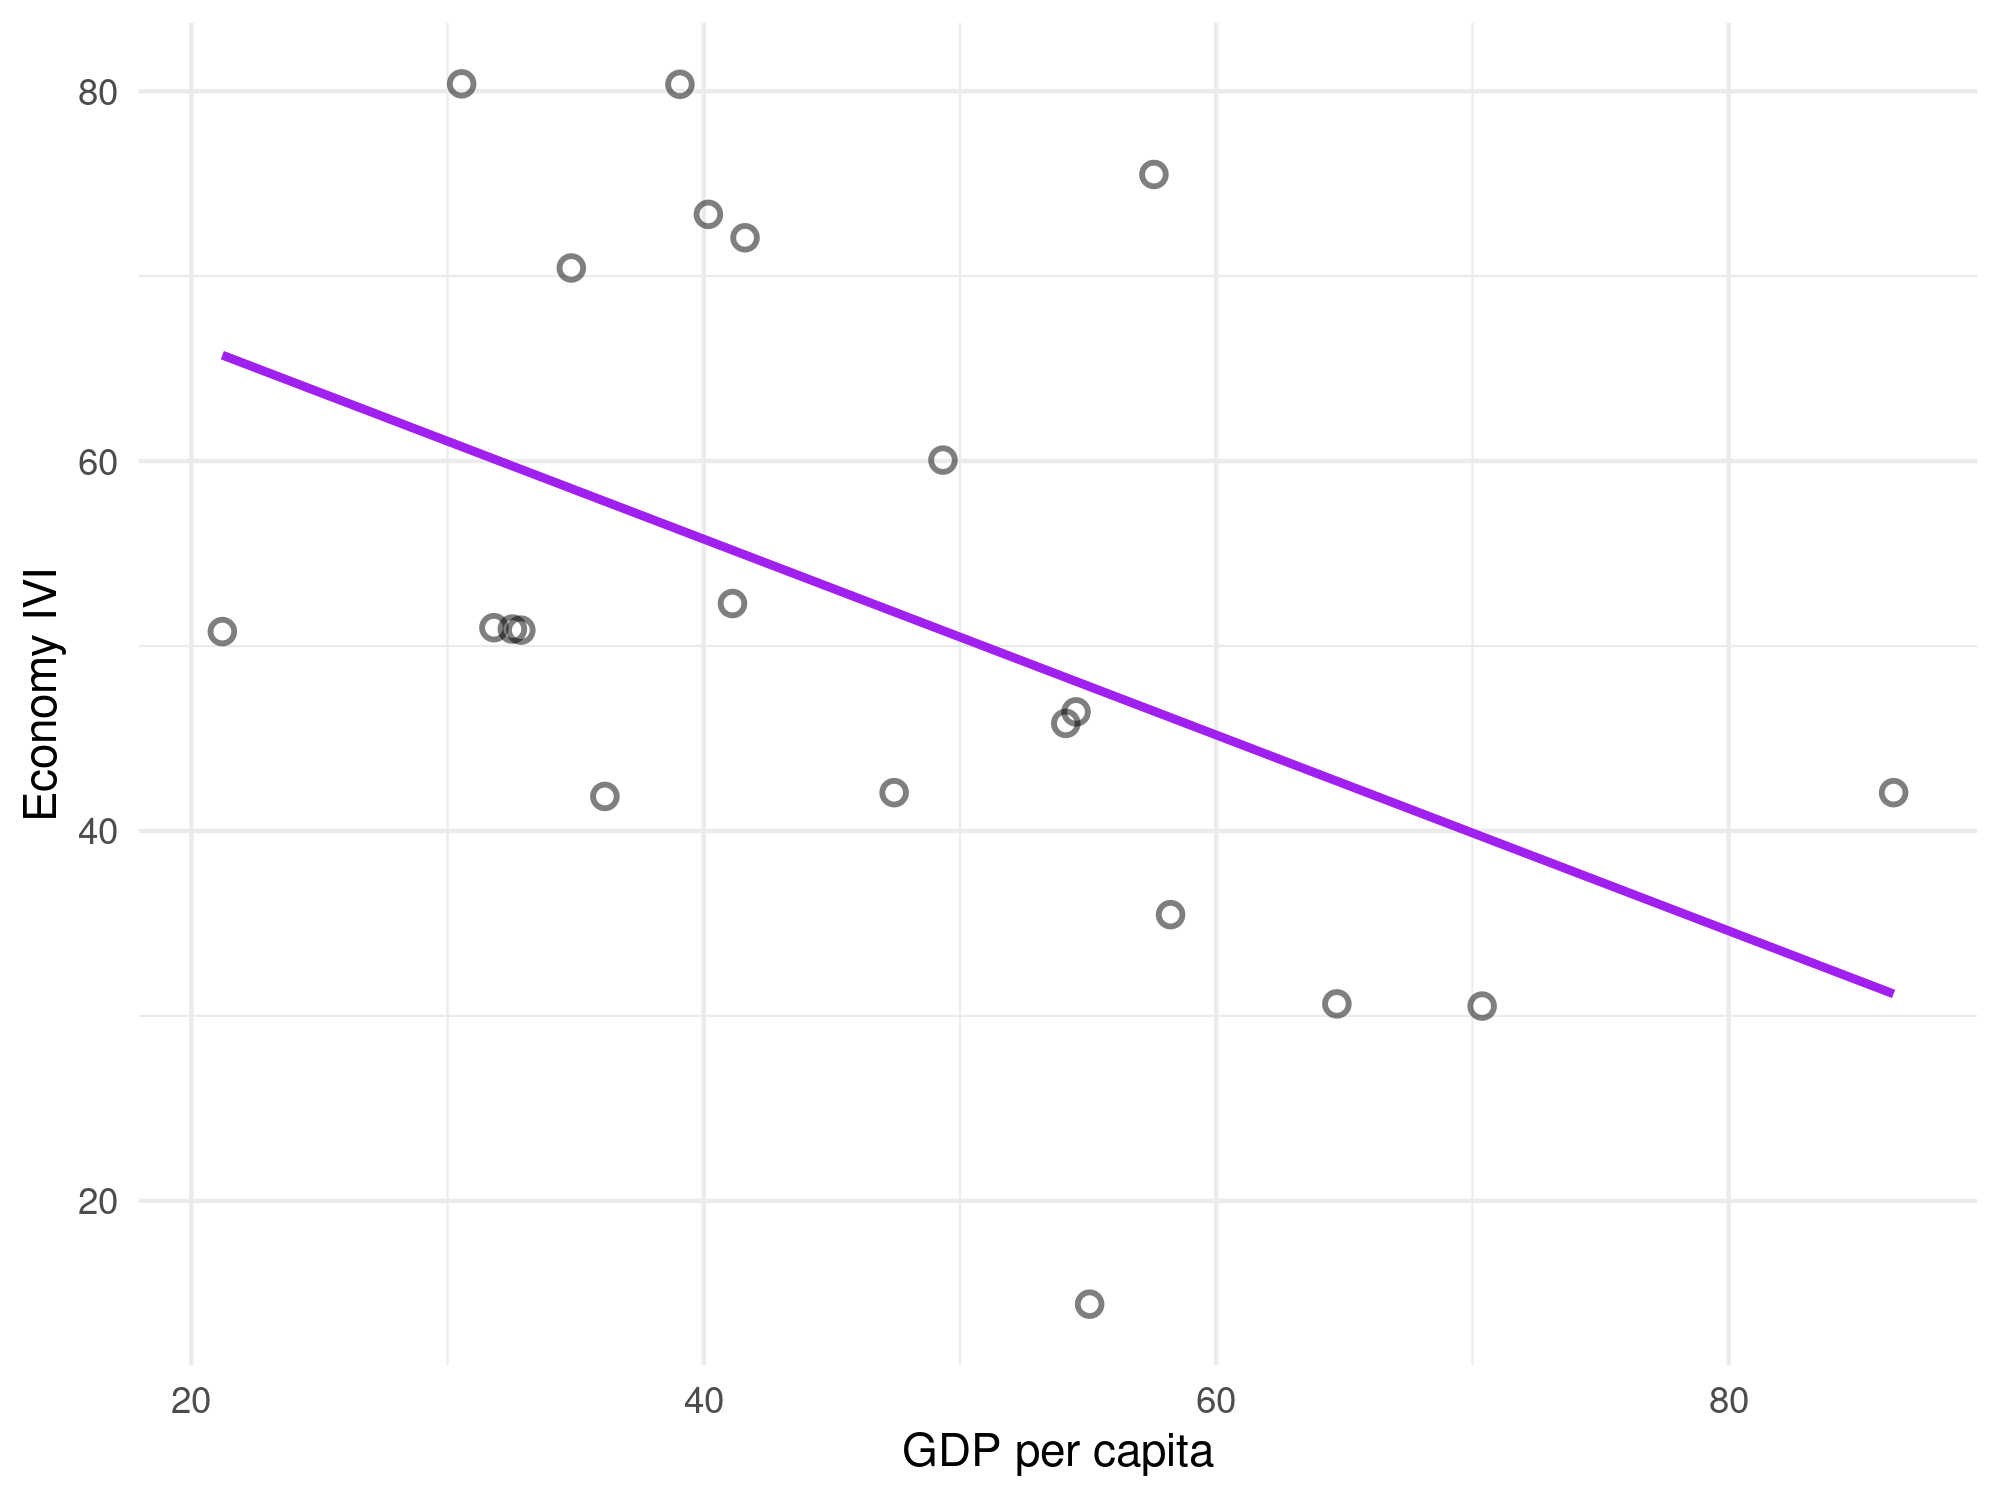
\includegraphics[width=0.5\paperwidth]{05-scatter-eco.png}
  \caption*{\hspace{-5cm}$r=-0.429 \quad p=0.02$}
\end{flushleft}

  \end{figure}
\end{frame}

% NEXT One is all remaining for scatterplots, add sig. and cor in caption

\section{Discussion}


\end{document}